%=====================================================================================================

%       Math 244 Lecture Notes

%       Chapter 20 Day Two

%				201701

%				LaTeX=>PDF sizing, graphics
%=====================================================================================================


\documentclass[12pt]{amsart}
\usepackage{amssymb,latexsym}
\usepackage{graphicx}
\usepackage{multicol}
\usepackage{multirow}
\usepackage{amsmath}
\usepackage{calc}
\usepackage{enumitem}
\usepackage{fancyhdr,lastpage}
\usepackage{setspace}
\usepackage{caption}
\usepackage{framed}
\usepackage{wasysym}

\theoremstyle{definition}
\pagestyle{fancy}
\newtheorem{theorem}{Theorem}
\newtheorem{lemma}{Lemma}
\newtheorem{defi}{Definition}
\newtheorem*{notation}{Notation}
\newtheorem{ex}{Example}
\newtheorem{proc}{Process}
\newtheorem{gw}{Group Work}
\newtheorem*{summary}{}

\setlength{\textwidth}{7.25in}			%for =>PDF, use 6.5in
\setlength{\textheight}{9.5in}		%for =>PDF, use 9.5in
\setlength{\oddsidemargin}{-0.375in}		
\setlength{\evensidemargin}{-0.375in}		
\setlength{\voffset}{-.75in}			%for=>PDF, use -0.75in
\setlength{\footskip}{15pt}


% For degree symbol
\newcommand{\degree}{\ensuremath{^\circ}}



% enumerate settings
\setlist{itemsep=4pt}	%topsep=0.1em
\renewcommand{\labelenumi}{ (\alph{enumi}) }			% makes enumeration (a) instead of (a).



\usepackage{placeins} % enables \FloatBarrier, useful for positioning figures/tables more precisely.
%\usepackage[dvips]{graphics}
%\usetikzlibrary{arrows}


\usepackage{pst-func}



\usepackage{hyperref}
%\usepackage{url}
\hypersetup{colorlinks=true,urlcolor=blue,linkcolor=blue,breaklinks=true}

\usepackage{xcolor}
%		My colors
\definecolor{silver}{rgb}{0.95,0.95,0.95}
\definecolor{mypurple}{cmyk}{0.5,1,0,0}			%purple
\definecolor{myblue}{cmyk}{1,0.012,0,0}		%blue
\definecolor{mygreen}{cmyk}{1,0,0.99995,0}		%green
\definecolor{myred}{cmyk}{0,1,1,0}


\setlength{\parindent}{0pt}

\date{}



\begin{document}

\newcommand{\ph}{\phantom}
\newcommand{\ds}{\displaystyle}

\renewcommand{\emph}{\textbf}
\onehalfspace

%============================================================
%           Header Stuff   CHANGE FOR EACH SECTION!!!
%============================================================

\fancyhf{}   % clears both header and footer
\fancyfoot[RE,RO]{ \scriptsize{Page \thepage\ of \pageref{LastPage}}}
\fancyfoot[LE,LO]{\scriptsize{Instructor:  J.Wherry}}
\fancyhead[RE,RO]{\scriptsize{Chapter 20 Day 2: Hypothesis Tests for One Average }}
\fancyhead[LE,LO]{\scriptsize{Math 244 Lecture Notes }}
\renewcommand{\headrulewidth}{0.4pt} % Removes header line if 0pt
\fancyfootoffset[LE,LO]{0in}        %Moves center ??
\renewcommand{\footrulewidth}{0.4pt} % Removes header line if 0pt



%============================================================
%           Title/ Info
%============================================================

\begin{center}

	\larger[3]	Math 244 Lecture Notes \smaller[3]		\\[22pt]

\end{center}

\section*{Chapter 20: Hypothesis Tests for One Average}




 \textbf{Overview:} We are continuing our investigation of averages. Last time, we did confidence intervals for a population mean ($\mu$). Today, we will test claims using hypothesis tests. We start with an overview of the H-test process.\\
 ~\\
  \begin{framed}
 \begin{enumerate}
 	\item State the Hypotheses. These will look something like the following: $$H_0:\text{parameter}=\#$$ $$H_A:\text{parameter} [<,>,\neq]\#$$
 	\item Determine the Model and Check Assumptions. 
 	\item Calculate the P-Value.
 	\item Conclusion. \end{enumerate}
 \end{framed}
 
 We are testing claims about $\mu$ so we will be using the CLT as our model:
 \begin{framed}
 The \emph{Central Limit Theorem} states that $$\bar{X}=$$ assuming that
 \begin{enumerate}
  \item \,
  \item \,
  \item \,
 \end{enumerate}
 \end{framed}

 The test will be remarkably similar to our 1-proportion z-test from a few weeks ago with a couple of minor exceptions.
 \begin{framed}
  $z$-scores are found by taking $z=\frac{value-center}{SD}$.
  
  $t$-scores are found by taking $t=\frac{value-center}{SE}$.
 \end{framed}
 ~\\
 We will look $t$-scores up using technology.
 \newpage
\begin{ex}
 It is claimed that Tylenol lasts for $4$ hours on average. After a clinical study involving $30$ randomly selected patients, Mr. Wherry is led to believe that the actual average is less than claimed. His data yields an average of $3.25$ hours with a standard deviation of $1$ hr. Test the claim!
\end{ex}
\noindent STEP I:
\vspace{0.5in}

\noindent STEP II:
\vspace{1.5in}

Assumptions?
\vspace{1in}

\noindent STEP III:
\vspace{2in}

Okay, we are a bit stuck, but let's do what we typically do. Draw a picture, find a z or t score, and look it up. Finally, let's use our calculator to help us from here.\\
~\\
\emph{TI-83 and TI-84:} [2nd]$\rightarrow$[Vars]$\rightarrow$[tcdf].\\
\emph{TI-89:} [Apps]$\rightarrow$[Stat/List]$\rightarrow$[F5:Dist]$\rightarrow$[tcdf].\\
~\\
The general setup is the same for all calculators. We need to type in ``tcdf(low t-score, high t-score, df)''.\\
~\\
Our P-value$=$\underline{\hspace{5in}}\\
~\\
\noindent STEP IV:

\newpage
\noindent Let's practice more with finding the area given $t$-scores.

\begin{ex}
 $P(t>2.31)$ if $df=15$
\end{ex}
\vspace{0.4in}

\begin{ex}
 $P(t\leq -1.5)$ if $n=31$
\end{ex}
\vspace{0.4in}

\begin{ex}
 $P(-1.96<t<1.96)$ if $n=10000$
\end{ex}
\vspace{0.4in}

\begin{ex}
 $P(x>10\,ft)$ if $\bar{x}=8\,ft$, $SE=\frac{s}{\sqrt{n}}=2\,ft$, and $n=31$
\end{ex}
\vspace{1.5in}

\begin{ex}
$P(152\,lb<x<160\,lb)$ if $\bar{x}=150\,lb$, $SE=\frac{s}{\sqrt{n}}=10\,lb$, and $n=16$
\end{ex}
\vspace{1.5in}
\begin{ex} Subway claims that their subs are $12$ inches long. A local woman tests $100$ subs and finds that their average is $11$ inches with a standard deviation of $2$ inches. Test the claim that the true average is LESS than claimed. If there is evidence of a difference, follow it up with a CI.
\end{ex}
\vfill
\newpage
\begin{ex} Claim: The average PCC student takes $13.2$ credits. Let's test it.\end{ex}
\vfill
\noindent \textbf{Checking work with Calculator:} In our calculator, we use ``tTest" to check our test. This is found in either [Stat]$\rightarrow$[Tests] on the TI-83/84 OR [Stat/List]$\rightarrow$[F6:tests] on the TI-89. Type in your relevant information and you are good to go!\\
~\\
Calc P-value:
\newpage
\begin{ex}
	The Oregon Zoo is curious how much on average people spend on food. A worker performs a survey and finds that out of $200$ people sampled (various days and times) that spent $\$10.72$ per person on average with a standard deviation of $\$1.35$. Test the claim that the average person spends $\$11$ or less.
\end{ex}

\begin{ex}
	The owners of Cinetopia want to know the average length of feature films. They sample $100$ movies from the last $4$ years and find that they have an average run length of $100\,mins$ with a standard deviation of $18\,mins$. Test the claim that the average movie length is different than $110$ minutes.
\end{ex}

\begin{ex}
	Barry Allen is training for the mile. In a recent study at STAR Labs, it was determined that he's running an average mile time of $0.1$ second with a standard deviation of $0.01$ seconds for a collection of $52$ samples. Using this information and assuming that his sample is representative, test the claim that Barry can run the mile in $0.11$ seconds or less.
\end{ex}

\begin{ex}
	Claire works as a night nurse. She samples $50$ individuals and finds that they have an average hospital bill of $\$3,200$ for one night with a standard deviation of $\$700$. Test the claim that it costs more than $\$3,000$ on average.
\end{ex}

\begin{ex}
	Mr. Wherry is training his cat, Fiona, for the Cat Olympics. She is known for her high jump. Curious as to what her true average high jump height is, Mr. Wherry measures several jump heights and gets the following data in feet: $4.5$, $4.75$, $4.75$, $4.8$, $4.8$, $4.8$, $4.8$, $5$, $5$, and $5.25$. Test the claim that the average is more than $4.7$ feet. [Picture included for educational purposes]
\end{ex}

\begin{figure}[h]
 \centering
 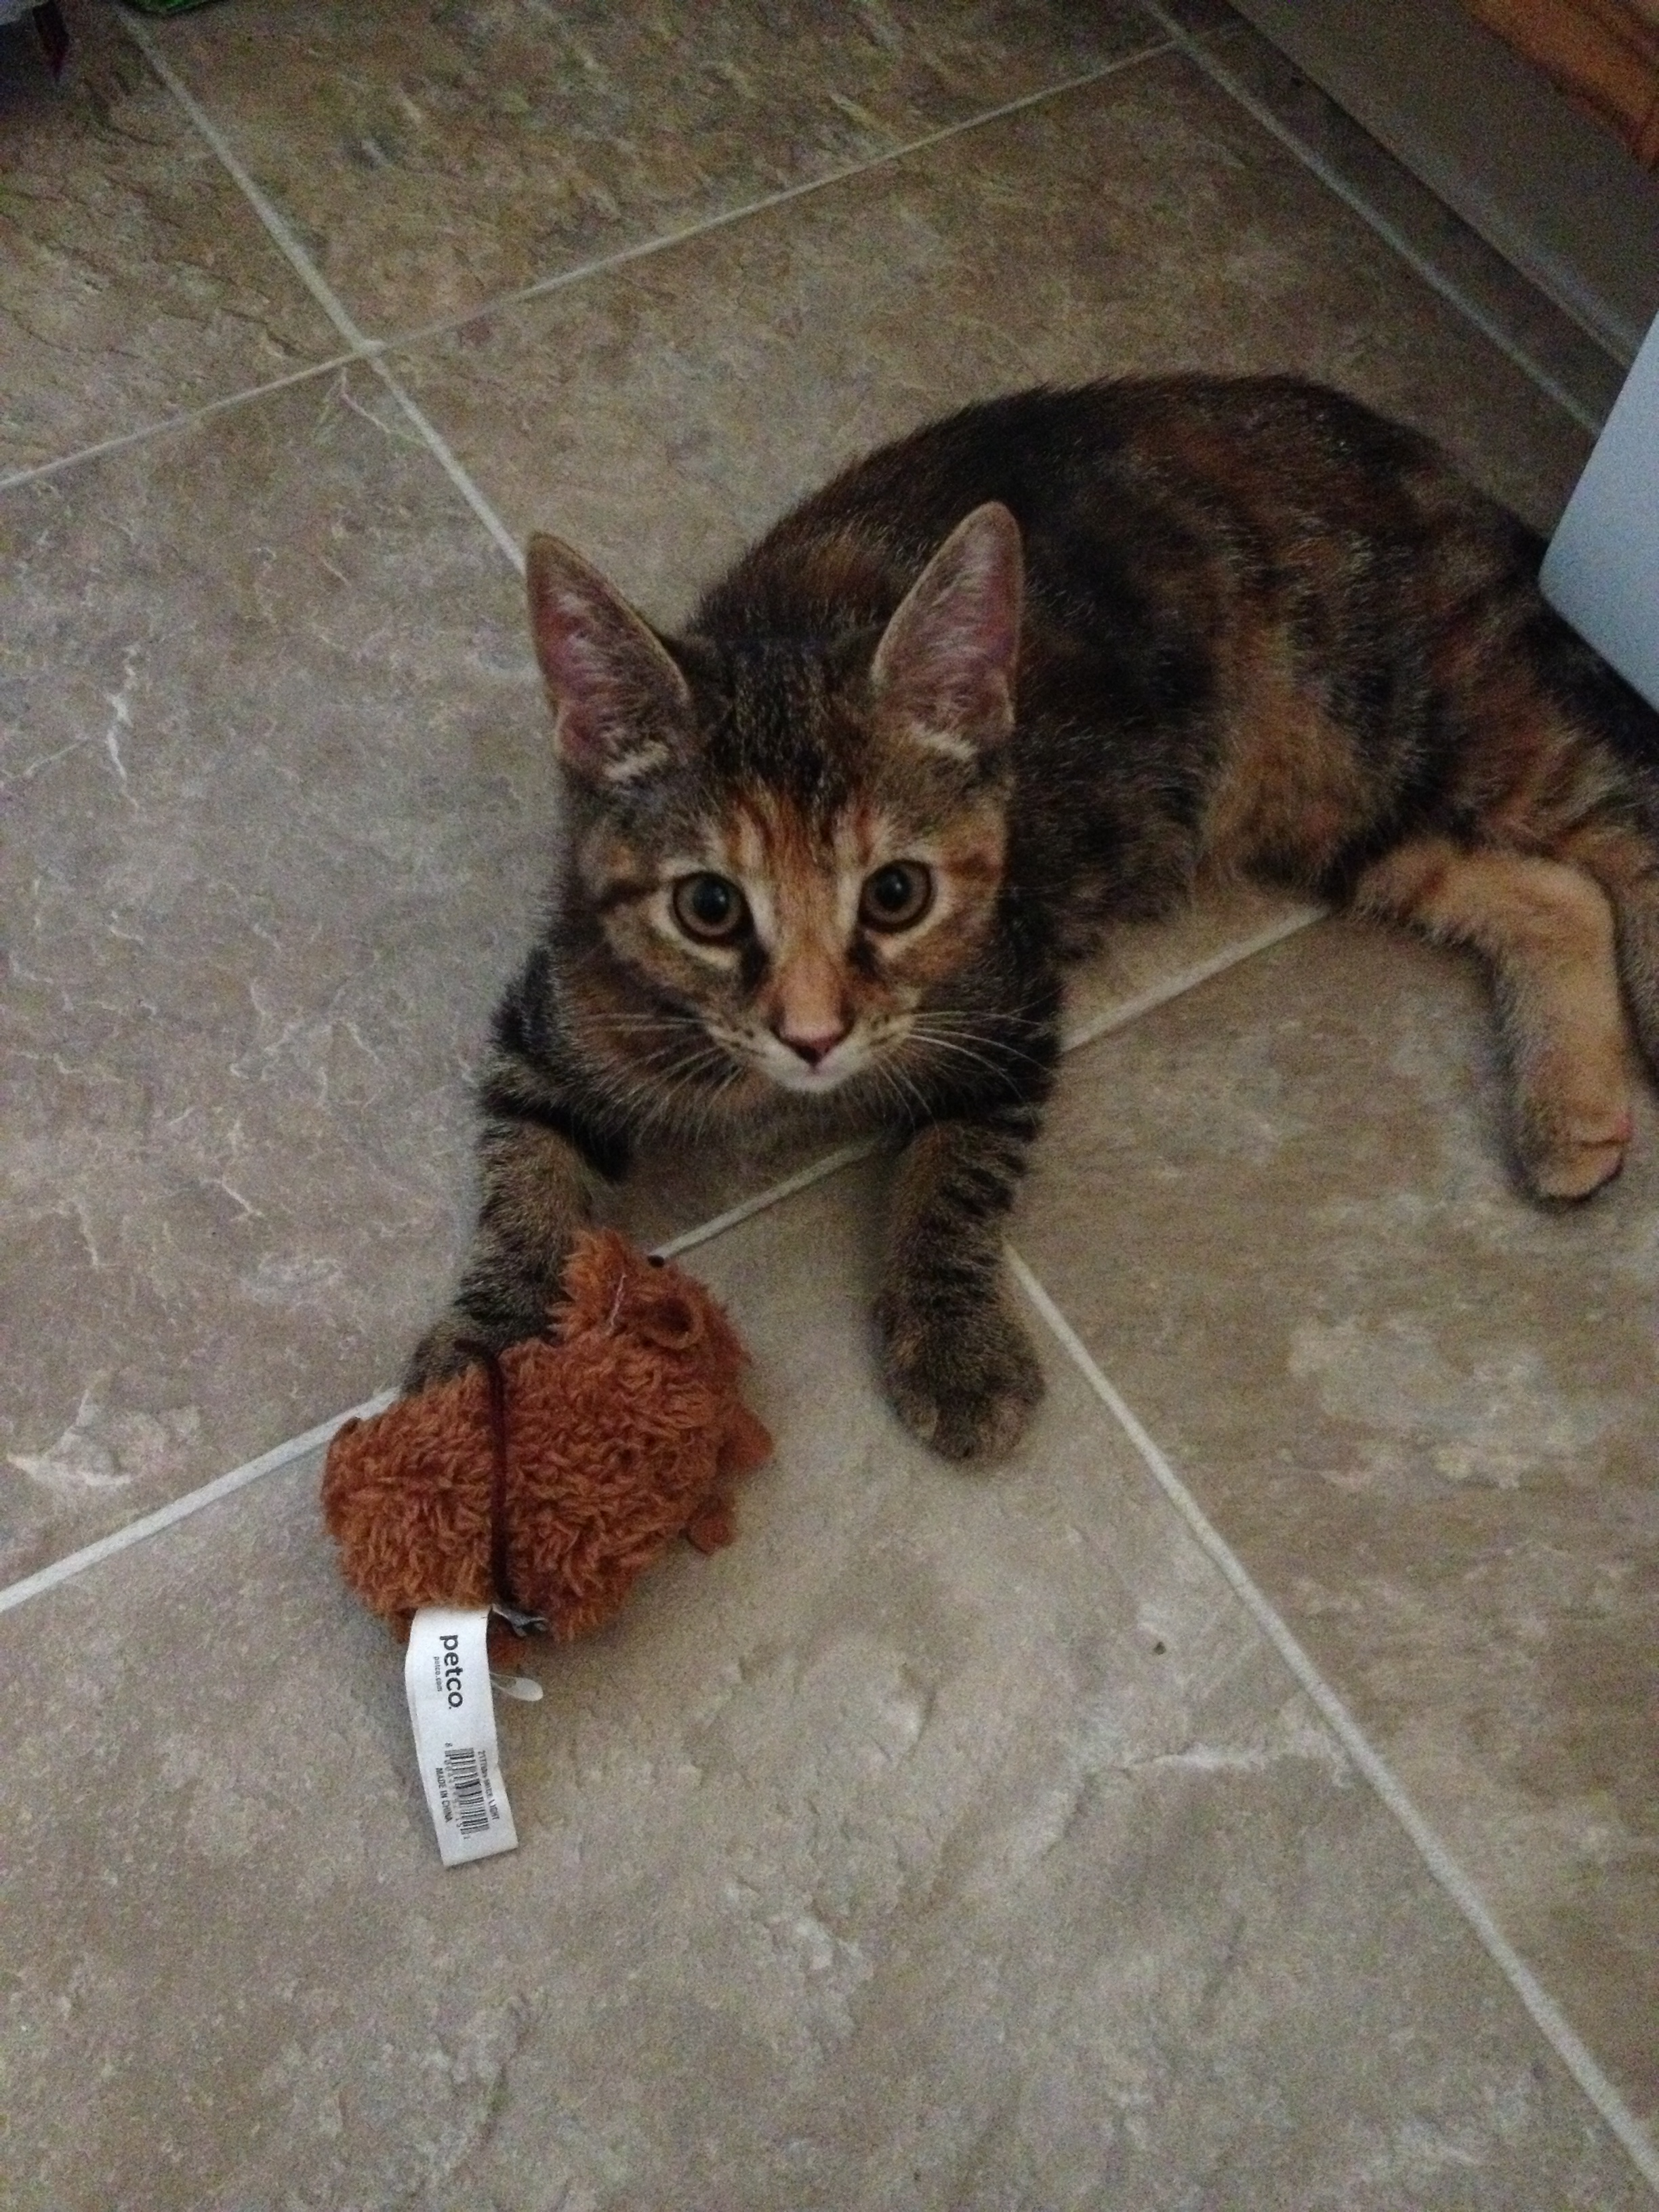
\includegraphics[width=2.5in,keepaspectratio=true]{./IMG_1011.JPG}
 % IMG_0929.JPG: 0x0 pixel, 0dpi, 0.00x0.00 cm, bb=
 \label{fig: Fiona and Chewie}
\end{figure}
\end{document}
